\documentclass[10pt]{article}
\usepackage[utf8]{inputenc}
\usepackage[T1]{fontenc}
\usepackage{a4wide}
\usepackage[version=4]{mhchem}
\usepackage{stmaryrd}
\usepackage{multicol}
\usepackage[export]{adjustbox}
\usepackage{hyperref}
\graphicspath{ {./images/} }
\hypersetup{colorlinks=true, linkcolor=blue, filecolor=magenta, urlcolor=cyan,}
\urlstyle{same}
\setlength\columnsep{25pt}

\title{WET - Water Efficiency Tool }

\author{
  Bessis, Hugoo\\
  ESILV\\
  Paris, France\\
  hugob6@orange.fr
  \and
  Saouab, Oumniya\\
  Al Akhawayn University\\
  Casablanca, Morocco\\
  oumniyasaouab@gmail.com
  \and
  Utama, Takara Izzah\\
  Hanyang University\\
  Seoul, South Korea\\
  takaraizzahutama@gmail.com
  \and
  van der Heide, Niklas\\
  ZHAW - School of Applied Sciences\\
  Winterthur, Switzerland\\
  niklasvdh@gmxch
}


\begin{document}
\maketitle

\begin{abstract}
House owners that have tight schedules or have a busy lifestyle tend to forget to monitor their houses properly. For example, they forget to close a water tap after using it. To check every water tap is closed properly or to make sure you are not using your water recklessly consumes time and requires a family member to be at the house. Therefore, our team is trying to develop an application (app) that monitors the water consumption in real time. The app not only provides real time monitoring but also provides users with consumption history, consumption limits, leakage detection, and consumption forecast. The primary goal of this app is to enable a user to monitor the water usage through a mobile application. This would help people structure their water usage more efficiently and change habits of consumption.
\end{abstract}

\clearpage

\begin{multicols}{2}

\section{Role Assignments}

\begin{itemize}
  \item User\\
  Users are people owning a home equipped appliances that include the necessary sensors and internet access. The User role should help the team better analyze what features are actually useful and to judge the current user experience.\\
  This role will be filled by Oumniya Saouab.
  \item Customer\\
  A home appliance company that wants to give their users the possibility to manage their appliances by using WET would be our customer. This role will help in creating a product that could actually be sold and generate profit.\\
  This role will be filled by Takara Utama.
  \item Software Developer\\
  The software developer thinks, designs, and realizes the software in general. Their goal is to implement all the requirements.\\
  This role will be filled by Niklas van der Heide.
  \item Development Manager\\
  Developer Manager is the person in charge of supervising their team's work throughout the app's development. They should have a good overview over what features are being worked on and by whom.\\
  This role will be filled by Hugo Bessis.
\end{itemize}

\iffalse
\begin{table}[!ht]
\centering
\begin{tabular}{| p{0.01\linewidth} | p{0.1\linewidth} | p{0.1\linewidth} |}
\hline
Role & Project Member & Description \\
\hline
User & Oumniya & Users are people owning a home equipped appliances that include the necessary sensors and internet access. The User role should help the team better analyze what features are actually useful and to judge the current user experience. \\
\hline
Customer & Takara & A home appliance company that wants to give their users the possibility to manage their appliances by using WET would be our customer. This role will help in creating a product that could actually be sold and generate profit. \\
\hline
Software Developer & Niklas & The software developer thinks, designs, and realizes the software in general. Their goal is to implement all the requirements. \\
\hline
Development Manager & Hugo & Developer Manager is the person in charge of supervising their team's work throughout the app's development. They should have a good overview over what features are being worked on and whom. by \\
\hline
\end{tabular}
\end{table}
\fi

\section{Introduction}
Managing water consumption is vital for life preservation. Better knowing one's water consumption at home can have a great impact on water saving. Even families could change habits of consumption. Reports have warned of an impending global water crisis due to surging population growth, climate change, reckless consumption, and chronic waste. We hope to help people to use water more responsibly to help stop the global water crisis. While trying to do some research on similar apps, we were not able to find that many existing projects. Thus, we are motivated to provide a solution to this problem.

Our application provides some features that help the user to monitor their water consumption in real time, let users know their consumption history based on day, weeks, etc. Also, the app let users limit their usage so that they could save water and money and even gave them the consumption forecast, so that they could change their habit if they are using water recklessly. As a result, we hope that this application will help the problem of the water crisis that is currently happening in the world right now.


\section{Problem Statement}
The Water Efficiency Tool is a project hoping to help people monitor and manage their water consumption. In this form we envision the application user to actively monitor their water consumption, and if there is any water running for an unusual duration the app will give you a notification about it, and you can remotely close the central water supply to make it stop. In other words, the Water Efficiency Tool is a project that aims to assist people in tracking and controlling their water usage. In its current form, the application allows users to actively monitor their water usage. If any water is left running for a length of time that is unusual, the app will notify the user and allow them to remotely shut off the main water supply to stop it.

Saving water or using water with responsibility is something that has been going on for years, but to actually do it or to encourage people to do so is a hard thing to do. Because excessive water use can go unnoticed. Water bills are relatively cheaper than other utilities. Compared to other problems, benefits of reducing water consumption are not necessarily felt by the individual. And many people don't believe that individual actions can make much of a difference compared to the amount of water lost through leakages. As a result, some other parts of the world are having a water crisis and shortage.


\section{Related Software}

\begin{enumerate}

  \item {Dropcountrer ${ }^{[1]}$}
  
  This app lets you know how much water you are using and sets benchmarks for conserving with this new web and mobile app that tracks water usage in real time and sends a usage warning to your device or smartphone if you're nearing overuse. In addition to that, the app connects to local utility companies and water districts to help users track water consumption. Adding to the daily tracking feature, the app sends users alerts on rebates and other preventative water-waste actions. App downloaders can also take advantage of the utility poke, which locates your water district and contacts them requesting user data.

  \item {Drip Detective ${ }^{[2]}$}
  
  Drip Detective is an application tells you how much water and money is going down the drain by timing leaks or measuring volume, then calculating the cost of your water leak by day, week, month, and year, in other words, by timing leaks or measuring volume, the application Drip Detective estimates how much water and money are being wasted. It then calculates the cost of your water leak by day, week, month, and year.

  \item {Klima ${ }^{[3]}$}
  
  Klima is a climate app that allows you to offset your emissions, reduce your carbon footprint and multiply your carbon impact. To do that, the app calculates a member's annual carbon footprint by asking them 9-10 lifestyle questions, including how they eat, whether they have a car, or how often they take a flight. These factors are used to calculate the user's estimated carbon footprint. It is not exatcly what our app will look like, but the purpose of the app is quite similar, which is trying to help the world.

  \item {Kill-Ur-Watts ${ }^{[4]}$}
  
  It is an application that permits residential customers to view, track, and manage their residential electricity use over time. This application utilizes common industry-based concepts and third-party data to empower residential users to make informed decisions on energy reduction strategies and implement common-sense energy efficiency improvements. Kill-Ur-Watts allows users to view hourly, daily, and monthly home energy consumption profiles and use social media outlets to challenge other users to reduce energy consumption. These 2 features are quite the same features that we are going to have on our application, which are to track our water consumption as well as our gamification, where we could share our achievement that we get for using water with responsibility to our social media.

  \item {Nest ${ }^{[5]}$}
  
  Nest is an app that lets you control the thermostat, alarm system, and camera. The approach of this app is quite similar to our app, which is trying to control the unused water. For example, from an unclosed water tap.

\end{enumerate}


\section{Requirements}

\begin{enumerate}
  \item {User Registration}
  
  A new user should be able to register themselves on the app. To do that they need to provide the following information:

  \begin{itemize}
    \item Full Name
  
    \item Address
  
    \item Country
  
    \item Phone Number
  
    \item Email
  
    \item Password
  
  \end{itemize}

  The user's email or phone number should be verified to ensure their authenticity. The set email or phone number together with the given password will be used to authenticate and login the user.

  \item {User Login}\\
  After a user has been successfully registered they should be able to log in to the app with their email or phone number together with the correct password. Only when logged in should the user be able to access, manage or change their home's information.

  \item {Device Registration} \\
  Home appliances that include the necessary wifi capability as well as the sensors to capture the information relevant to the system should be able to be registered in the app. To add a new device, the user must be logged in and connected to the same network as the appliance to be added.
  
  \item {Modifying unit and language settings} \\
  The user should be able to modify the unit settings. For the volume of water, the user can change the metric by liter, cubic meter or gallons. The user can also choose which currency to display, and the app language.
  \item {Real Time Monitoring} \\
  A user should be able to monitor their water consumption in real time. The App should be able to display what devices are currently using up water and at what rate. This would give the user the comfort of knowing that there is no unexpected or wasteful water usage.
  \item {Consumption History} \\
  The App should display and visualize the homes past water usage over different time periods:

  \begin{itemize}
    \item 1 day
  
    \item 1 Week
  
    \item 1 Month
  
    \item 1 Year
  
    \item All
  
  \end{itemize}

  The user should be presented with the hard numbers as well as visual representations in the form of charts and graphs.

  \item {Consumption Limits}\\
  To help the user save water and money, they should be able to set a limit for the time frames:

  \begin{itemize}
    \item daily limit
  
    \item weekly limit
  
    \item monthly limit
  
  \end{itemize}
  
  They should be able to set the limits based on the amount of water or cost.
  
  Once a limit is reached, the user should be notified of that.


  \item {Leakage Detection} \\
  The Application should alert the user if an appliance is using up water for an unusual duration or at an irregular rate.
  
  \item {Remote Control} \\
  When leaving for a longer duration of time, the user should be able to remotely close the central water supply to not use any water. If appliances can be separately disabled, the user should be able to disable them separately. \\
  If any water is used despite the appliance or the central water supply is dissabled, the user should be notified.

  \item {Consumption Forecast} \\
  This feature helps the user to predict its water consumption for the next week. When the user clicks on this, they should be able to see the volume of water they will most likely consume the next week based on the previous week's water consumption.

  The user can also click on the cost prediction button that will display the predicting cost of their water consumption for the next week based on their previous week's water consumption.

  The user can also select the time frame of the prediction and get either a week, a month or a year prediction.

  This feature will help the user to adapt its consumption to prevent over consumption usage of water.

  \item {Gamification} \\
  When the user is clicking on the badges button, it will display all the badges and achievements they made using the apps. These can be earned by using the app through the time. The badges and achievements will reward the user for consuming water responsibly, according to government laws and international recommendations (COP21, GIEC, etc.). The user will be able to share their achievements and badges on social media such as Twitter, Instagram and Meta.

\end{enumerate}


\section{Development environment}

\begin{enumerate}
  \item {OS} \\
  We are going to develop applications on Windows using mac OS and Windows as our main development platform. Windows is a good choice for programming since it provides many programs, language, and also has a really good IDE, Visual Studio. And the whole Windows development stack is amazing. However, MacOS is also a good option for someone that works on a back-end server because it's based on Unix and runs nearly all Linux software.
  
  \item {Services} \\
  One Service that will be used is a server hosting provider. The backend software, as well as the database would be hosted online.
  
  \item {Languages} \\
  We have decided to use $G O$ to create an API to manage a $S Q L$ database. For the main application, Flutter and Dart were selected. With Flutter, a cross platform application is possible.
  
  \item {Development Environment}

  \begin{itemize}
    \item {Visual Studio Code}
    
    Our application will be launched on multiple platforms, and Visual Studio Code offers that feature. Visual Studio Code has an in-built debugger making the development flow less ‘clicky’ and maintains a single view with the code and debugger. In addition to this, there is intelliSense built into the code editor which is a form of predictive coding. With the addition of framework, library, and language plugin extensions, we can fully utilize the usage of it.

    \item {Android Studio} \\
    
    Since our application will also run in Android, we decided to work with Android Studio for the front-end. Android Studio picks the changes in the code as soon as there is one. This change is seen without restarting the app or without rebuilding your app. This makes our development way faster and easier.

    \item {GitHub} \\

    GitHub is an online software development platform. It\textquotesingle s used for storing, tracking and collaborating on software projects. It makes it easy for our team to share code files and make some issues regarding the code

  \end{itemize}
  
  
  \item {Software In Use} \\
  Since we have not yet started development, we have not yet used any software. The following software will probably be used:

  \begin{itemize}
    \item Database Management

    \item Mobile Phone Emulator

  \end{itemize}
\end{enumerate}


\section{Specification}

\begin{enumerate}
  \item {User Login Page} \\
  When the user opens the app, he will get the login page. They can either create a new account by choosing the register option, or login if they already have an account. \\
  To log in, the user must fill in their mail address or phone number, and password. They can also check the "Remember me" mark to stay connected every time the app is closed and reopened. \\
  \begin{center}
    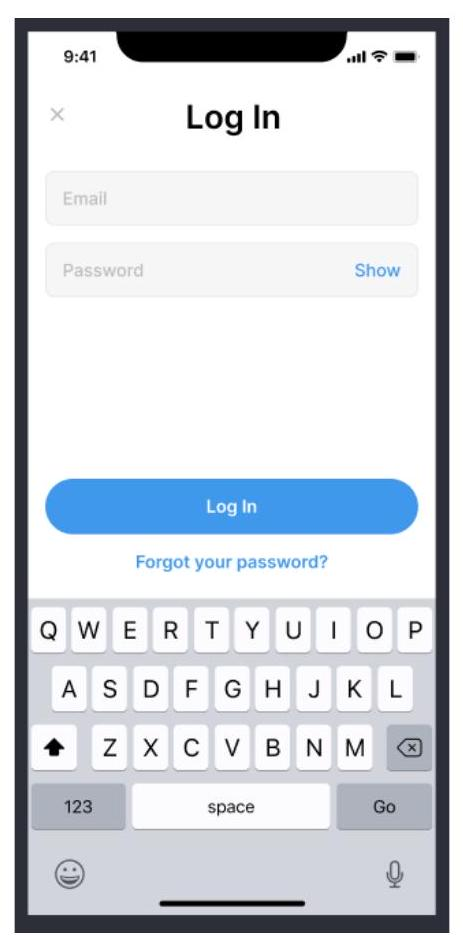
\includegraphics[max width=4cm]{login.jpg}
  \end{center}
  
  \item {User Registration Page} \\
  When choosing the register option on the login page, the user should be asked to fill in personal information such as:
  \begin{itemize}
    \item full name
  
    \item home address
  
    \item country of residence
  
    \item phone number
  
    \item email
  
    \item a password
  
  \end{itemize}

  They will receive a SMS and email confirmation to confirm the creation of their account.
  
  \begin{center}
    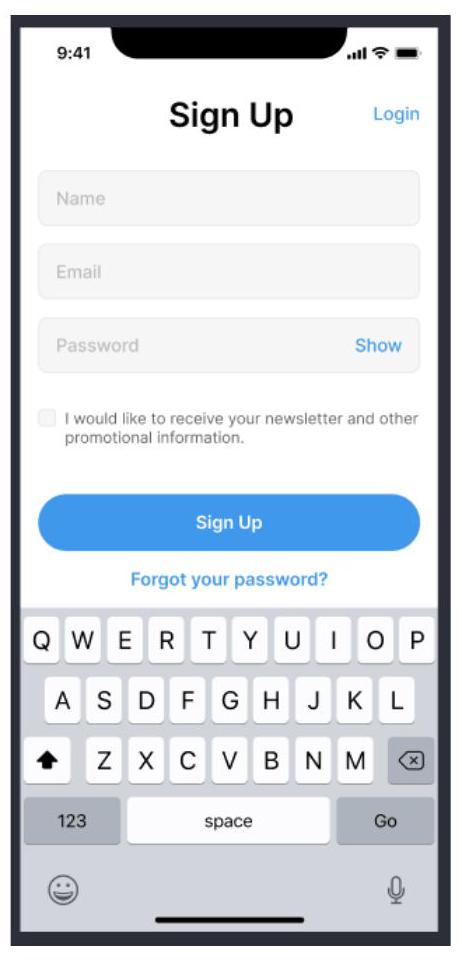
\includegraphics[max width=4cm]{signup.jpg}
  \end{center}

  \item {House Registration Page} \\
  After logging in for the first time or by choosing the "register devices" option on the profile settings page, the user will be asked to register their home appliance devices into the app.\\
  In order to do that, the user has to be connected to each appliance's personal Wi-Fi network. After the connection has been established the app will automatically find all the compatible devices connected. The user can manually change the name of the device to create a more enjoyable experience. We found that the technical name of most devices do not properly describe their function.

  \begin{center}
    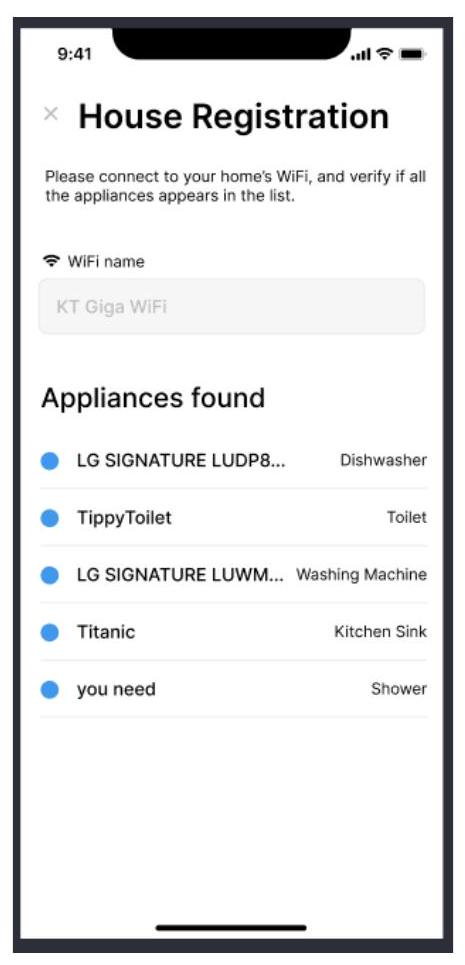
\includegraphics[max width=4cm]{houseregistration.jpg}
  \end{center}

  \item {Main Page} \\
  After finishing registering everything and or logining in, the user will be shown the main page. On this page, the app will display a statistical overview of the relevant happenings. This overview should include:
  
  \begin{itemize}
    \item That days water usage
  
    \item Appliance status
  
    \item Overview if daily, weekly or monthly usage goals have been failed or how far away from failing the user is.
  
  \end{itemize}
  
  The days water usage should be shown as a percentage of the set usage goal. A circle should be filled up with $100 \%$ filled representing $100 \%$ of the goal reached.
  
  \begin{center}
    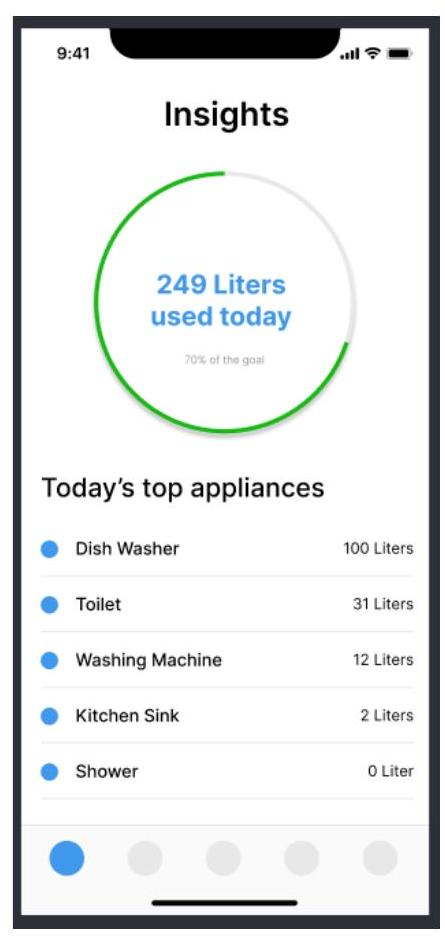
\includegraphics[max width=4cm]{mainpage-1.jpg}
  \end{center}

  Should the user's set goal be failed, the graph that displays the percentage of the goal reached should also reflect that.
  
  \begin{center}
    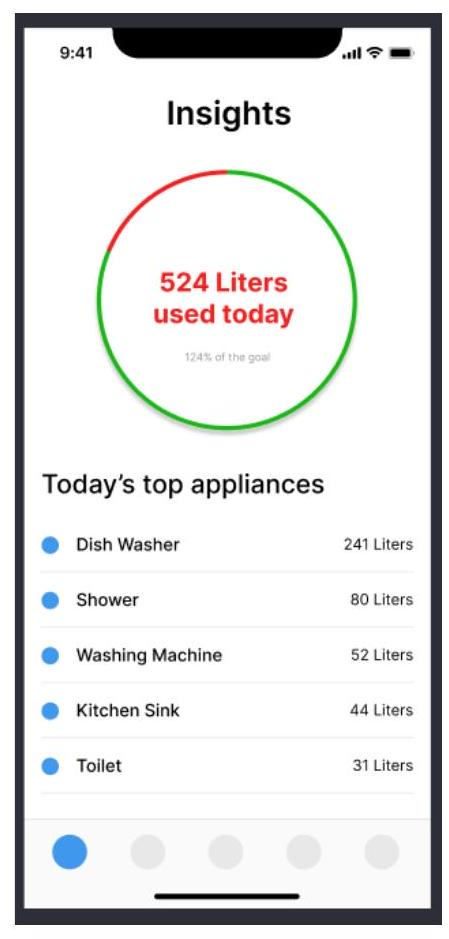
\includegraphics[max width=4cm]{mainpage-2.jpg}
  \end{center}

  \item {Consumption History and Forecast Page} \\
  In the Consumption History and Forecast Page, the user will see a line chart showing water consumption over a selected time frame. The user can modify the time frame of the chart:

  \begin{itemize}
    \item current day

    \item current week

    \item current month

  \end{itemize}

  At the bottom of the page there is a list of all appliances. The user is able to click on each device to show the consumption of only the selected device over the selected time period.

  On the same page the current water consumption is extrapolated and an estimated consumption for the selected time period is calculated. Should the estimated water consumption be higher than the set consumption goal, the user is warned of that.

  In the list of all appliances at the bottom of the page the current status of each appliance is visible. If an appliance is currently running the status should be "active" if not, "inactive". For "active" devices their current rate of consumption is also noted in the form of liters per minute.

  All numbers are rounded to the first decimal.

  \begin{center}
    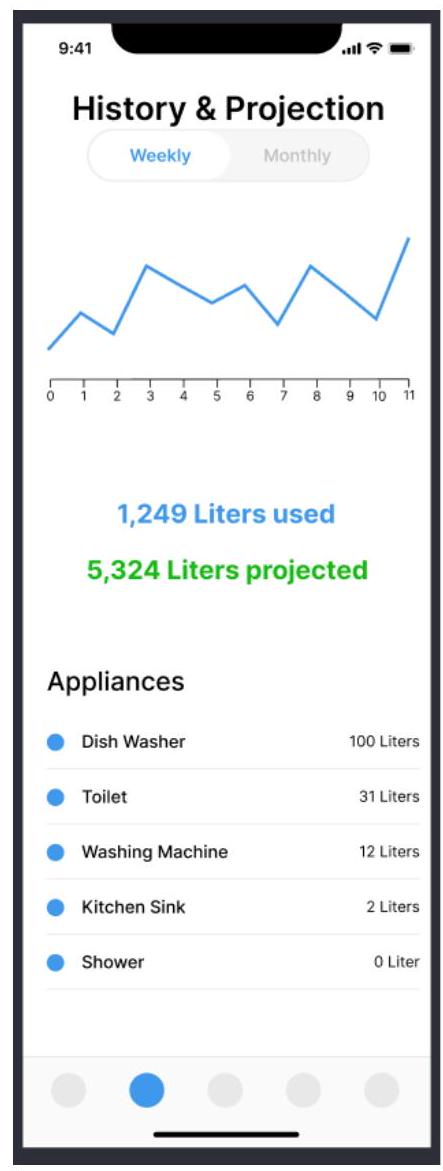
\includegraphics[max width=4cm]{historyandprojection.jpg}
  \end{center}

  \item {Holiday Mode Page} \\
  On the Holiday Mode Page the user is able to set their whole house to "holiday mode". If the home is in "holiday mode" the user is automatically notified if any water is used up at irregular amounts. On the same page, the idea of holiday mode is explained to the user.

  \begin{center}
    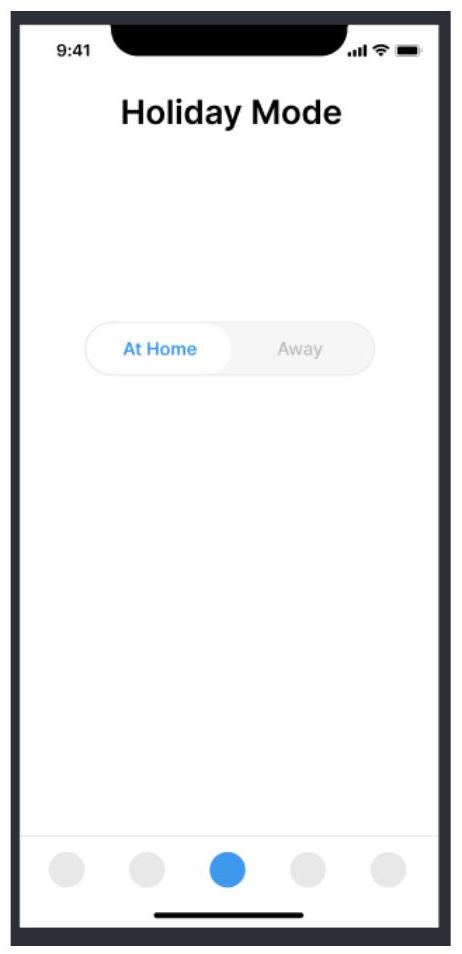
\includegraphics[max width=4cm]{holidaymode.jpg}
  \end{center}

  \item {Notifications Page} \\
  On the Notification Page the user is presented with all previous notifications. If a notification has not yet been seen by the user, it is marked as "unread".

  \begin{center}
    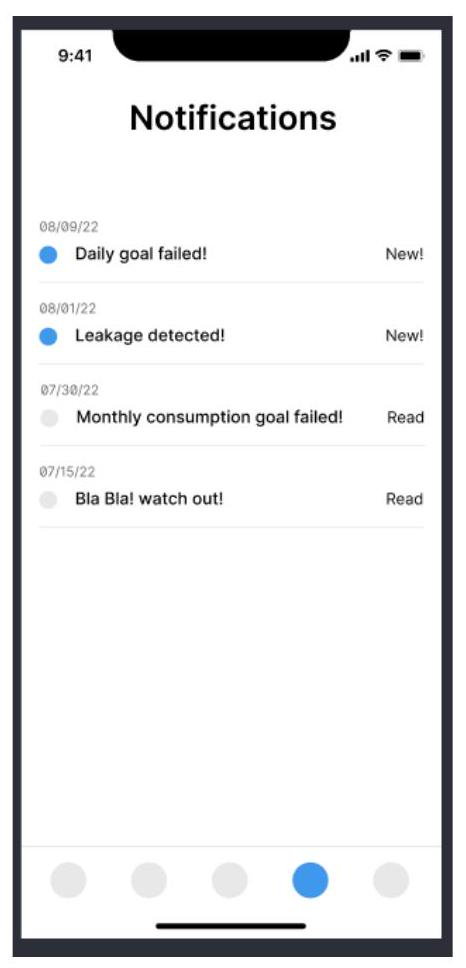
\includegraphics[max width=4cm]{notifications.jpg}
  \end{center}

  \item {Profile Settings Page} \\
  After registering a new account, the user will have to select some settings according to its country and metrics regulation, such as litter, cubic meter or gallons for the volume metric. They also have to choose the language they want to use as well as the currency such as US dollar, Euro, KRW, etc. for cost estimates.

  The Profile Settings Page also allows the user to set their consumption goal. This number is the amount of water to be consumed in a month. The unit is the one selected by the user and the number is an integer.

  The option to delete the users account can also be found a t the bottom of the Profile Settings Page.

  \begin{center}
    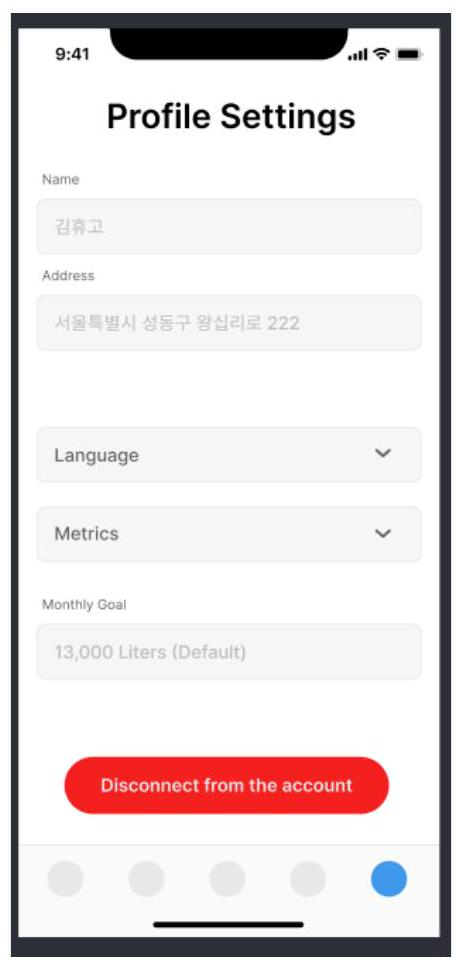
\includegraphics[max width=4cm]{profilesettings.jpg}
  \end{center}

  \item {Navigation Bar}
  On the bottom of the app, the user can click on different icons that are lined up side to side. Each icon takes the user to a page specified above.
  \begin{itemize}
    \item {Main Page}
    \item {Consumption History and Forecast Page}
    \item {Holiday Mode Page}
    \item {Profile Settings Page}
  \end{itemize}

\end{enumerate}

\end{multicols}

\clearpage
\section{Citations}
[1] "Dropcountr." Dropcountr, \href{https://www.dropcountr.com/}{https://www.dropcountr.com/}

[2] "Drip Detective." DevPost, \href{https://devpost.com/software/drip-detective}{https://devpost.com/software/drip-detective}

[3] "Klima." Klima, \href{https://klima.com/}{https://klima.com/}

[4] "Kill-Ur-Watts", DevPost, \href{https://appsforenergy.devpost.com/submission}{https://appsforenergy.devpost.com/submission}

[5] “Nest.", Nest, \href{http://www.nest.com}{www.nest.com}

\end{document}